% Two lifetimes of a shared source (Fig. 2). Build: xelatex fig_lifetimes.tex.
% One recipient with two readers; where each release policy frees the slot. Text in Carlito
% (metric-compatible with the Calibri of the plots).
\documentclass[border=0pt]{standalone}
\usepackage{fontspec}
\setmainfont{Carlito}
\usepackage{tikz}
\usepackage{pifont}
\usetikzlibrary{arrows.meta}

\definecolor{ink}{HTML}{1F2933}\definecolor{sub}{HTML}{5F6B7A}\definecolor{line}{HTML}{9AA5B1}
\definecolor{bimD}{HTML}{1F4E8C}\definecolor{bimA}{HTML}{3A73C0}
\definecolor{rsD}{HTML}{2E6B34}\definecolor{rsT}{HTML}{DDEEDB}
\definecolor{pvD}{HTML}{3A73C0}\definecolor{pvT}{HTML}{DCE7F6}
\definecolor{frD}{HTML}{B07A12}\definecolor{frA}{HTML}{E9B23A}\definecolor{frT}{HTML}{F8E3AE}\definecolor{frF}{HTML}{FFF6DF}
\definecolor{coral}{HTML}{C8414B}
\newcommand{\fs}[1]{\fontsize{#1}{#1}\selectfont}
\newcommand{\var}[1]{\textit{#1}}

\begin{document}
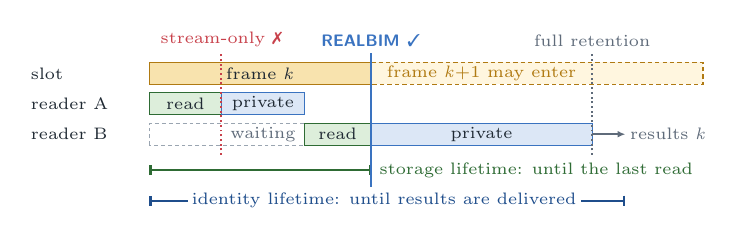
\begin{tikzpicture}[x=1pt,y=1pt,font=\fs{6.4},text=ink]
\useasboundingbox (0,5) rectangle (252,72.5);
% time positions: publish, A's read ends, B's read ends (last read), outputs complete, axis end
\def\xp{44}\def\tA{70}\def\tB{124}\def\tO{204}\def\xe{250}
\def\tbar#1#2#3#4#5{\draw[#4,fill=#5,line width=.45pt] (#1,#3-4) rectangle (#2,#3+4);}

% row labels
\foreach \y/\t in {56/slot,45/reader A,34/reader B}{\node[anchor=west,inner sep=0pt,font=\fs{6.5}] at (1,\y) {\t};}

% the slot: frame k, then the next frame once the borrow is returned
\tbar{\xp}{\tB}{56}{frD}{frT}
\node at ({(\xp+\tB)/2},56) {frame \var{k}};
\draw[frD,fill=frF,line width=.45pt,dash pattern=on 1.6pt off 1.1pt] (\tB,52) rectangle (\xe-6,60);
\node[text=frD] at ({(\tB+\tO)/2},56) {frame \var{k}{+}1 may enter};

% reader A reads first; reader B has not started when A's read completes
\tbar{\xp}{\tA}{45}{rsD}{rsT}\node at ({(\xp+\tA)/2},45) {read};
\tbar{\tA}{\tB-24}{45}{pvD}{pvT}\node at ({(\tA+\tB-24)/2},45) {private};
\draw[line,line width=.45pt,dash pattern=on 1.4pt off 1.1pt] (\xp,30) rectangle (\tB-24,38);
\node[text=sub] at ({(\tA+\tB-24)/2},34) {waiting};
\tbar{\tB-24}{\tB}{34}{rsD}{rsT}\node at ({\tB-12},34) {read};
\tbar{\tB}{\tO}{34}{pvD}{pvT}\node at ({(\tB+\tO)/2},34) {private};
\draw[-{Latex[length=2.8pt,width=2.4pt]},sub,line width=.6pt] (\tO,34) -- (\tO+12,34);
\node[anchor=west,inner sep=0pt,text=sub] at (\tO+13.5,34) {results \var{k}};

% the two lifetimes
\draw[rsD,line width=.75pt,{Bar[width=3.6pt]}-{Bar[width=3.6pt]}] (\xp,21) -- (\tB,21);
\node[anchor=west,inner sep=0pt,text=rsD] at (\tB+3,21) {storage lifetime: until the last read};
\draw[bimD,line width=.75pt,{Bar[width=3.6pt]}-{Bar[width=3.6pt]}] (\xp,10) -- (\tO+12,10);
\node[anchor=east,inner sep=0pt,text=bimD,fill=white,inner xsep=1.5pt] at (\tO-4,10) {identity lifetime: until results are delivered};

% where each policy frees the slot
\draw[coral,densely dotted,line width=.7pt] (\tA,26.5) -- (\tA,63.5);
\draw[bimA,line width=.8pt] (\tB,15) -- (\tB,63.5);
\draw[sub,densely dotted,line width=.7pt] (\tO,26.5) -- (\tO,63.5);
\node[anchor=south,inner sep=0pt,text=coral,font=\fs{6.2}] at (\tA,65.5) {stream-only \ding{55}};
\node[anchor=south,inner sep=0pt,text=bimA,font=\fs{6.2}\bfseries] at (\tB,65.5) {\textsf{REALBIM} \ding{51}};
\node[anchor=south,inner sep=0pt,text=sub,font=\fs{6.2}] at (\tO,65.5) {full retention};
\end{tikzpicture}
\end{document}
